% % def.tex

% File containing LaTeX macros.
% Has grown by accretion; can be better organized.

\documentclass{article}
\usepackage{amsmath}
\usepackage{amssymb}
\usepackage{bm}
\usepackage{graphicx}
\usepackage{epstopdf}
\DeclareGraphicsRule{.tif}{png}{.png}{`convert #1 `basename #1 .tif`.png}
\usepackage{color}
\usepackage{pdfsync}
\pagestyle{plain}

%\pagestyle{empty}

\textheight 9 true in
\textwidth 6.5 true in
\hoffset -.75 true in
\voffset -.75 true in
 \mathsurround=2pt  \parskip=2pt
\def\crv{\cr\noalign{\vskip7pt}}

\def\a{\alpha } \def\b{\beta } \def\d{\delta } \def\D{\Delta } \def\e{\epsilon }
\def\g{\gamma } \def\G{\Gamma} \def\k{\kappa} \def\l{\lambda } \def\L{\Lambda }
\def\th{\theta } \def\Th{\Theta} \def\r{\rho} \def\o{\omega} \def\O{\Omega}
\def\ve{\varepsilon}

\def\sA{{\cal A}} \def\sB{{\cal B}} \def\sC{{\cal C}} \def\sE{{\cal E}} \def\sI{{\cal I}}
\def\sR{{\cal R}} \def\sF{{\cal F}} \def\sG{{\cal G}} \def\sM{{\cal M}}
\def\sT{{\cal T}} \def\sH{{\cal H}} \def\sD{{\cal D}} \def\sW{{\cal W}}
\def\sL{{\cal L}} \def\sP{{\cal P}} \def\s{\sigma } \def\S{\Sigma}
\def\sU{{\cal U}} \def\sY{{\cal Y}}

\def\gm{\gamma -1}
\def\summ{\sum_{j=1}^4}

\def\bb{{\bm b}} \def\yb{{\bm y}}
\def\ub{{\bm u}}  \def\xb{{\bm x}} \def\vb{{\bm v}} \def\wb{{\bm w}}
\def\omegab{{\bm \omega}} \def\rb{{\bm r}} \def\ib{{\bm i}} \def\jb{{\bm j}}
\def\lb{{\bm l}} \def\kb{{\bm k}} \def\Ab{{\bm A}} \def\fb{{\bm f}} \def\Ub{{\bm U}}
\def\Fb{{\bm F}} \def\nb{{\bm n}} \def\Db{{\bm D}} \def\eb{{\bm e}}
\def\gb{{\bm g}}  \def\hb{{\bm h}} \def\Yb{{\bm Y}} \def\Rb{{\bm R}}

\def\As1{{\bf {\cal A}}_1}\def\DO{{\cal D}_0} \def\UO{{\cal U}_0}
\def\ie{{\it{i.e.}}}

\def\ubbar{{\bf {\bar{u}}}} \def\sbar{{\bar{\sigma }}} \def\ubar{{\bar{u}}}
\def\abar{{\bar{a}}} \def\vbar{{\bar{v}}}  \def\rbar{{\bar{\rho}}}
\def\pbar{{\bar{p}}} \def\ebar{{\bar{e}}} \def\Tbar{{\bar{T}}}
\def\bbar{{\bar{\beta}}} \def\Mbar{{\bar{M}}}  \def \sMbar{{\bar{\cal M}}}
\def\Ebar{{\bar{E}}} \def\sMbar{{\bar{\cal M}}}
\def\sPbar{{\bar{\cal P}}} \def\xbar{{\bar{x}}}

\newcommand{\pdv}[2]{\frac{\partial#1}{\partial#2}}
\newcommand{\dv}[2]{\frac{d#1}{d#2}}
\newcommand{\ord}[2]{#1^{(#2)}}
\newcommand{\vct}[1]{\vec{#1}}

 \newcommand{\bc}{\begin{center}}
 \newcommand{\ec}{\end{center}}

 \newcommand{\bq}{\begin{equation}}
 \newcommand{\eq}{\end{equation}}

 \newcommand{\beqs}{\begin{eqnarray}}
 \newcommand{\eeqs}{\end{eqnarray}}

 \newcommand{\beqa}{\begin{eqnarray*}}
 \newcommand{\eeqa}{\end{eqnarray*}}

 \newcommand{\ol}{\overline}
 \newcommand{\ul}{\underline}

 \newcommand{\dint}{{\int \!\! \int \!\!}}
 \newcommand{\tint}{{\int \!\! \int \!\! \int \!\!}}

 \newcommand{\bfig}{\begin{figure}}
 \newcommand{\efig}{\end{figure}}

 \newcommand{\cen}{\centering}
 \newcommand{\n}{\noindent}

 \newcommand{\btab}{\begin{table}}
 \newcommand{\etab}{\end{table}}

 \newcommand{\btbl}{\begin{tabular}}
 \newcommand{\etbl}{\end{tabular}}

 \newcommand{\bdes}{\begin{description}}
 \newcommand{\edes}{\end{description}}

 \newcommand{\benum}{\begin{enumerate}}
 \newcommand{\eenum}{\end{enumerate}}

 \newcommand{\bite}{\begin{itemize}}
 \newcommand{\eite}{\end{itemize}}

 \newcommand{\cle}{\clearpage}
 \newcommand{\npg}{\newpage}

 \newcommand{\bss}{\begin{singlespace}}
 \newcommand{\ess}{\end{singlespace}}

 \newcommand{\bhalf}{\begin{onehalfspace}}
 \newcommand{\ehalf}{\end{onehalfspace}}

 \newcommand{\bds}{\begin{doublespace}}
 \newcommand{\eds}{\end{doublespace}}

 \newcommand{\eps}{\mbox{$\epsilon$}}
 \newcommand{\stilde}{\mbox{$\tilde s$}}
 \newcommand{\shat}{\mbox{$\hat s$}}

 \newcommand{\blue}{\color{blue}}
 \newcommand{\red}{\color{red}}
 \newcommand{\magenta}{\color{magenta}}
 \newcommand{\green}{\color{green}}
 \newcommand{\nc}{\normalcolor}



\def\arg{{\rm{arg}}}
\def\Arg{{\rm{Arg}}}
\def\imath{i}
\def\Log{{\rm{Log}}}
\def\erfc{{\rm{erfc}}}
\def\Oh{\mathcal{O}}
\def\oh{\mathsf{o}}

\def\Res{{\rm{Res}}}

\def\fl{{\rm{fl}}}

\def\Xint#1{\mathchoice
{\XXint\displaystyle\textstyle{#1}}%
{\XXint\textstyle\scriptstyle{#1}}%
{\XXint\scriptstyle\scriptscriptstyle{#1}}%
{\XXint\scriptscriptstyle\scriptscriptstyle{#1}}%
\!\int}
\def\XXint#1#2#3{{\setbox0=\hbox{$#1{#2#3}{\int}$ }
\vcenter{\hbox{$#2#3$ }}\kern-.6\wd0}}
\def\ddashint{\Xint=}
\def\dashint{\Xint-}

%\numberwithin{equation}{section}

% def.tex

% File containing LaTeX macros.
% Has grown by accretion; can be better organized.

\documentclass{article}
\usepackage{amsmath}
\usepackage{amssymb}
\usepackage{bm}
\usepackage{graphicx}
\usepackage{epstopdf}
\DeclareGraphicsRule{.tif}{png}{.png}{`convert #1 `basename #1 .tif`.png}
\usepackage{color}
\usepackage{pdfsync}
\pagestyle{plain}

%\pagestyle{empty}

\textheight 9 true in
\textwidth 6.5 true in
\hoffset -.75 true in
\voffset -.75 true in
 \mathsurround=2pt  \parskip=2pt
\def\crv{\cr\noalign{\vskip7pt}}

\def\a{\alpha } \def\b{\beta } \def\d{\delta } \def\D{\Delta } \def\e{\epsilon }
\def\g{\gamma } \def\G{\Gamma} \def\k{\kappa} \def\l{\lambda } \def\L{\Lambda }
\def\th{\theta } \def\Th{\Theta} \def\r{\rho} \def\o{\omega} \def\O{\Omega}
\def\ve{\varepsilon}

\def\sA{{\cal A}} \def\sB{{\cal B}} \def\sC{{\cal C}} \def\sE{{\cal E}} \def\sI{{\cal I}}
\def\sR{{\cal R}} \def\sF{{\cal F}} \def\sG{{\cal G}} \def\sM{{\cal M}}
\def\sT{{\cal T}} \def\sH{{\cal H}} \def\sD{{\cal D}} \def\sW{{\cal W}}
\def\sL{{\cal L}} \def\sP{{\cal P}} \def\s{\sigma } \def\S{\Sigma}
\def\sU{{\cal U}} \def\sY{{\cal Y}}

\def\gm{\gamma -1}
\def\summ{\sum_{j=1}^4}

\def\bb{{\bm b}} \def\yb{{\bm y}}
\def\ub{{\bm u}}  \def\xb{{\bm x}} \def\vb{{\bm v}} \def\wb{{\bm w}}
\def\omegab{{\bm \omega}} \def\rb{{\bm r}} \def\ib{{\bm i}} \def\jb{{\bm j}}
\def\lb{{\bm l}} \def\kb{{\bm k}} \def\Ab{{\bm A}} \def\fb{{\bm f}} \def\Ub{{\bm U}}
\def\Fb{{\bm F}} \def\nb{{\bm n}} \def\Db{{\bm D}} \def\eb{{\bm e}}
\def\gb{{\bm g}}  \def\hb{{\bm h}} \def\Yb{{\bm Y}} \def\Rb{{\bm R}}

\def\As1{{\bf {\cal A}}_1}\def\DO{{\cal D}_0} \def\UO{{\cal U}_0}
\def\ie{{\it{i.e.}}}

\def\ubbar{{\bf {\bar{u}}}} \def\sbar{{\bar{\sigma }}} \def\ubar{{\bar{u}}}
\def\abar{{\bar{a}}} \def\vbar{{\bar{v}}}  \def\rbar{{\bar{\rho}}}
\def\pbar{{\bar{p}}} \def\ebar{{\bar{e}}} \def\Tbar{{\bar{T}}}
\def\bbar{{\bar{\beta}}} \def\Mbar{{\bar{M}}}  \def \sMbar{{\bar{\cal M}}}
\def\Ebar{{\bar{E}}} \def\sMbar{{\bar{\cal M}}}
\def\sPbar{{\bar{\cal P}}} \def\xbar{{\bar{x}}}

\newcommand{\pdv}[2]{\frac{\partial#1}{\partial#2}}
\newcommand{\dv}[2]{\frac{d#1}{d#2}}
\newcommand{\ord}[2]{#1^{(#2)}}
\newcommand{\vct}[1]{\vec{#1}}

 \newcommand{\bc}{\begin{center}}
 \newcommand{\ec}{\end{center}}

 \newcommand{\bq}{\begin{equation}}
 \newcommand{\eq}{\end{equation}}

 \newcommand{\beqs}{\begin{eqnarray}}
 \newcommand{\eeqs}{\end{eqnarray}}

 \newcommand{\beqa}{\begin{eqnarray*}}
 \newcommand{\eeqa}{\end{eqnarray*}}

 \newcommand{\ol}{\overline}
 \newcommand{\ul}{\underline}

 \newcommand{\dint}{{\int \!\! \int \!\!}}
 \newcommand{\tint}{{\int \!\! \int \!\! \int \!\!}}

 \newcommand{\bfig}{\begin{figure}}
 \newcommand{\efig}{\end{figure}}

 \newcommand{\cen}{\centering}
 \newcommand{\n}{\noindent}

 \newcommand{\btab}{\begin{table}}
 \newcommand{\etab}{\end{table}}

 \newcommand{\btbl}{\begin{tabular}}
 \newcommand{\etbl}{\end{tabular}}

 \newcommand{\bdes}{\begin{description}}
 \newcommand{\edes}{\end{description}}

 \newcommand{\benum}{\begin{enumerate}}
 \newcommand{\eenum}{\end{enumerate}}

 \newcommand{\bite}{\begin{itemize}}
 \newcommand{\eite}{\end{itemize}}

 \newcommand{\cle}{\clearpage}
 \newcommand{\npg}{\newpage}

 \newcommand{\bss}{\begin{singlespace}}
 \newcommand{\ess}{\end{singlespace}}

 \newcommand{\bhalf}{\begin{onehalfspace}}
 \newcommand{\ehalf}{\end{onehalfspace}}

 \newcommand{\bds}{\begin{doublespace}}
 \newcommand{\eds}{\end{doublespace}}

 \newcommand{\eps}{\mbox{$\epsilon$}}
 \newcommand{\stilde}{\mbox{$\tilde s$}}
 \newcommand{\shat}{\mbox{$\hat s$}}

 \newcommand{\blue}{\color{blue}}
 \newcommand{\red}{\color{red}}
 \newcommand{\magenta}{\color{magenta}}
 \newcommand{\green}{\color{green}}
 \newcommand{\nc}{\normalcolor}



\def\arg{{\rm{arg}}}
\def\Arg{{\rm{Arg}}}
\def\imath{i}
\def\Log{{\rm{Log}}}
\def\erfc{{\rm{erfc}}}
\def\Oh{\mathcal{O}}
\def\oh{\mathsf{o}}

\def\Res{{\rm{Res}}}

\def\fl{{\rm{fl}}}

\def\Xint#1{\mathchoice
{\XXint\displaystyle\textstyle{#1}}%
{\XXint\textstyle\scriptstyle{#1}}%
{\XXint\scriptstyle\scriptscriptstyle{#1}}%
{\XXint\scriptscriptstyle\scriptscriptstyle{#1}}%
\!\int}
\def\XXint#1#2#3{{\setbox0=\hbox{$#1{#2#3}{\int}$ }
\vcenter{\hbox{$#2#3$ }}\kern-.6\wd0}}
\def\ddashint{\Xint=}
\def\dashint{\Xint-}

%\numberwithin{equation}{section}


\begin{document}

\bc Alexander Garcia \hfill May 30, 2017 \\ Assignment-1\ec

\bigskip

\benum

% Problem 1 ----------------------------------------------------------------------------------------------------
\item Let $f(x) = e^{x}\cos {2x}.$
\benum
\item

	The definition of the Taylor polynomial is as follows:

	$$T_n(x) = \sum_{k=0}^{n}{\frac{(x-x_0)^k}{k!}f^{(k)}(x_0)}$$

	In this case, $n=4$, and $x_0 = 0$.

	We start by finding $f^{(1)}(x), f^{(2)}(x), f^{(3)}(x)$, and $f^{(4)}(x)$ \\

	$f^{(1)}(x) = -2e^xsin(2x)+e^xcos(2x) = e^x(cos(2x)-2sin(2x))$

	$f^{(2)}(x) = e^x(-2sin(2x)-4cos(2x))+e^x(cos(2x)-2sin(2x)) = -e^x(4sin(2x)+3cos(2x))$

	$f^{(3)}(x) = -e^x(8cos(2x)-6sin(2x)) - e^x(4sin(2x)+3cos(2x)) = e^x(2sin(2x)-11cos(2x))$

	$f^{(4)}(x) = e^x(4cos(2x)+2sin(22sin(2x)) + e^x(2sin(2x)-11cos(2x)) = e^x(24sin(2x)-7cos(2x))$ \\

	Evaluating these functions at the center point, we get: \\

	$f(0) = e^0cos(0) = 1$

	$f^{(1)}(0) = e^0(cos(0)-2sin(0)) = 1$

	$f^{(2)}(0) = -e^0(4sin(0)+3cos(0)) = -3$

	$f^{(3)}(0) = e^0(2sin(0)-11cos(0)) = -11$

	$f^{(4)}(0) = -e^0(24sin(0)-7cos(0) = -7$ \\

	We now have all the pieces we need to determine the polynomial expansion. \\

	$$P_n(x) = \frac{x^0}{0!} f(0) + \frac{x^1}{1!} f^{(1)}(0) + \frac{x^2}{2!} f^{(2)}(0) +
	\frac{x^3}{3!} f^{(3)}(0) + \frac{x^4}{4!} f^{(4)}(0)$$

	$$= 1+x-\frac{3}{2} x^2 - \frac{11}{6} x^3 - \frac{7}{24} x^4$$ \\


\item

	By definition, the derivitive form of the remainder is

	$$R_n(x) = \frac{(x-x_0)^{n+1}}{(n+1)!} f^{(n+1)}(c)$$

	where $c$ is close to $x_0$.

	In this case, we have $n=4, x_0 = 0$ from the previous question.

	\newpage

	$R_n(x) = \frac{x^5}{5!}f^{(5)}(c)$

	$f^{(5)}(c) = e^x(48cos(2x) + 14sin(2x)) + e^x(24sin(2x) - 7cos(2x))$

	$= e^x(41cos(2x)+38sin(2x))$]$_{x=c}$ \\

	Therefore,

	$$R_4(x) = \frac{x^5}{120} e^c(41cos(2c)+38sin(2c))$$ \\

\item

	We know the remainder, $R_4(x)$ from part (c). Given a closed interval, we can find the maximum error by
	finding the maximum remainder in this interval. To do this, we must find its derivative,
	whose zeroes will show all maxima and minima.

	$f^{(6)}(x) = e^x(-82sin(2x)+76cos(2x)) + e^x(41cos(2x) + 38sin(2x)) = e^x(117cos(2x) - 44sin(2x))$ \\

	Now find zeroes.

	$e^x(117cos(2x)-44sin(2x)) = 0$

	$117cos(2x)-44sin(2x) = 0$

	$\frac{117}{44} = \frac{sin(2x)}{cos(2x)}$

	$x = \frac{1}{2} tan^{-1}(\frac{117}{44}) \approx 0.606$ \\

	Our candidate points are then $\{-\frac{\pi}{4}, 0.606, \frac{\pi}{4} \}$ \\

	$f^{(5)}(\frac{\pi}{4}) = 38*e^{\frac{\pi}{4}} \approx 83.3$

	$f^{(5)}(-\frac{\pi}{4}) = -38*e^{\frac{\pi}{4}}$

	$f^{(5)}(0.606) = e^{0.606}(41cos(2*0.606)+38sin(2*0.606)) \approx 91.6$ \\

	As $f^{(5)}(0.606)$ is clearly the max, this is what we use for determining the error bound. \\

	$$max(R_4(x)) = \frac{(\frac{\pi}{4})^5}{5!}*91.6$$

	$$\approx 0.228$$

\newpage

\item

Figure \ref{fig:graph1} shows the actual function compared to its $4^{th}$ degree Taylor expansion over the range
$x \in [\frac{-\pi}{4} , \frac{\pi}{4} ]$. Figure \ref{fig:graph2} shows the maximum error between the two, which
agrees with the upper bound calculated in part (c).

\begin{figure}[h!]
	\centering
	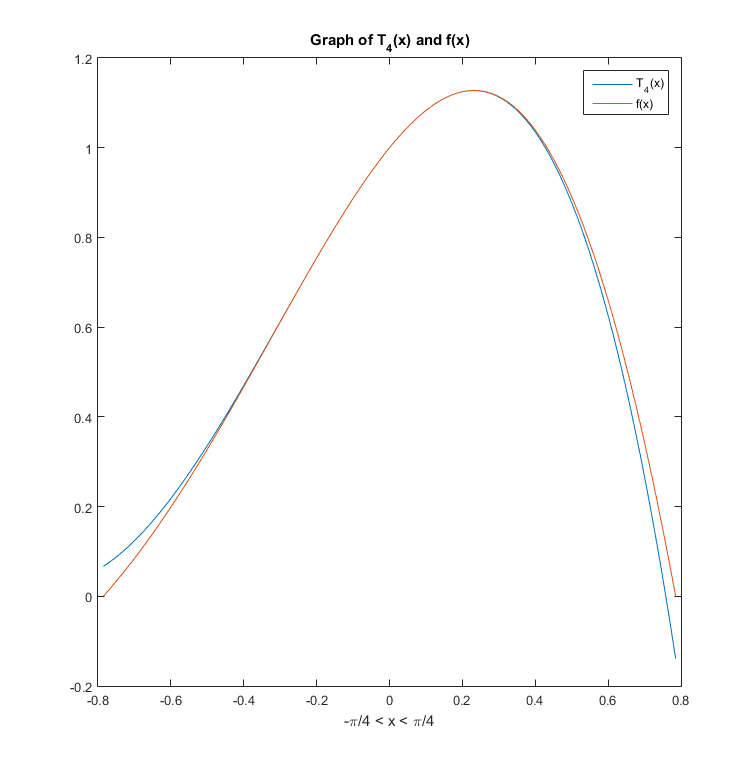
\includegraphics[width=4in, height=3.5in]{tf.png}
	\caption{Taylor expansion and initial function}
	\label{fig:graph1}
\end{figure}

\begin{figure}[!h]
	\centering
	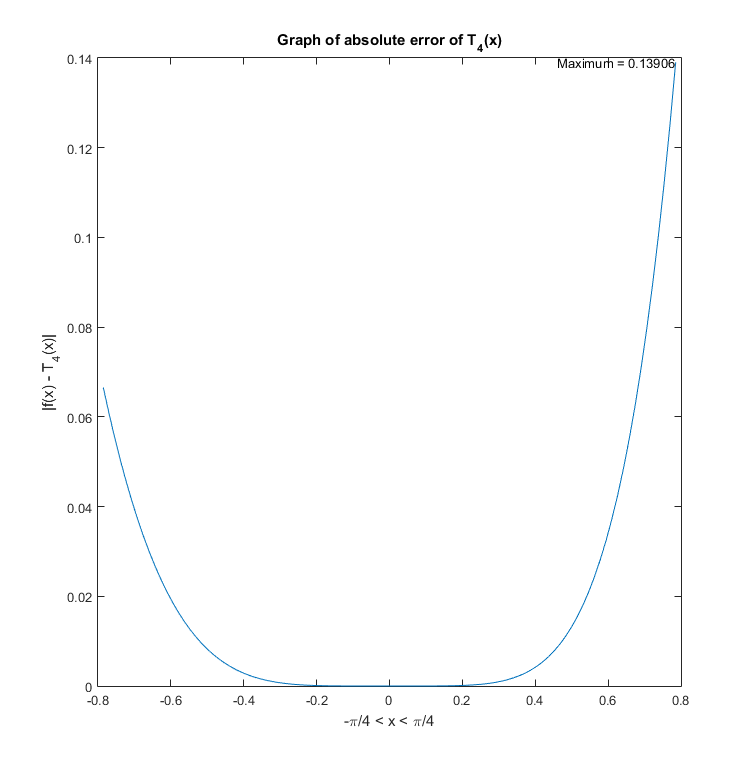
\includegraphics[width=4in, height=3.5in]{abs_error.PNG}
	\caption{Difference between the Taylor expansion and the initial function}
	\label{fig:graph2}
\end{figure}

\eenum

% Problem 2
\item

	$b = 10.\overline{110}_2$
	$= 2^1 + (0.\overline{110})_2$

	$z = 0.\overline{110}_2$

	$z = 0.110\overline{110})2$

	$2^3*z = 110.\overline{110}_2 = 2^2 + 2^1 + z$

	$8z = 6+z$

	$z = \frac{6}{7}$

	$b_{10} = 2 + z_{10} = 2 + \frac{6}{7} = \frac{18}{7} = 2.\overline{857142}$

% Problem 3
\item


	$6.7_{10}$

	$6_{10} = 110_2$

	\begin{tabular}{ll}

		$\frac{14}{10} = d_1 + \frac{d_2}{2} + \cdots$ & $ d_1 = 1$ \\

		$\frac{4}{5} = d_2 + \frac{d_3}{2} + \cdots$ & $d_2 = 0$ \\

		$\frac{8}{5} = d_3 + \frac{d_4}{2} + \cdots$ & $d_3 = 1$ \\

		$\frac{6}{5} = d_4 + \frac{d_5}{2} + \cdots$ & $d_4 = 1$ \\

		$\frac{2}{5} = d_5 + \frac{d_6}{2} + \cdots$ & $d_5 = 0$ \\

		$\frac{4}{5} = d_6 + \frac{d_7}{2} + \cdots$ & $d_6 = 0$ \\

	\end{tabular} \\

	The value generating $d_6$ is the same as the one generating $d_2$, and thus we are in a loop generating
	the repeating pattern 0110.

	$6.7_{10} = 110.1\overline{0110}_2 = 1.101\overline{0110}*2^2$

	The IEEE representation of this number designates one signed bit (in this case it is 0, as 6.7>0), 8 for the exponent (in this case 2),
	and 23 for the mantissa (in this case $101\overline{0110}$. The $23^{rd}$ digit of the mantissa is 0, so the number is truncated when
	stored.

	The exponent that is stored is the real exponent + a bias, which in this case is 127.

	$fl(6.7)$ is stored in the machine as

	\begin{center}
	\begin{tabular}{c | c | c}

		$0$ & $10000001$ & $10101100110011001100110$ \\

		sign & exponent + bias & mantissa \\

	\end{tabular} \\
\end{center}

	Converting the stored number back to decimal gives us $2^{129-127} * q$

	$q = 1 + 2^{-1} + 2^{-3} + 2^{-5} + 2^{-6} + 2^{-9} + 2^{-10} + 2^{-13} + 2^{-14} + 2^{-17} + 2^{-18}+2^{-21} + 2^{-22} \approx 1.675$

	$fl(6.7) = 2^2 * q  \approx (6.7+1.90735*10^{-7})$

	The relative error $d = \frac{6.7-fl(6.7)}{6.7} = 2.84679*10^{-8}$

	$\epsilon_{mach}$ for a 32 bit float is $\frac{1}{2^{23}} \approx 1.19*10^{-7}$

	$\frac{1}{2} * \epsilon_{mach} \approx 5.96 * 10^{-8}$

	More importantly, $$\frac{1}{2} * \epsilon_{mach} \leq d$$ \\

% Problem 4
\item (Pencil-and-paper and MATLAB)
Holmes 1.5(a).

% Problem 5
\item (Pencil-and-paper and MATLAB)
Holmes 1.12.

% Problem 6
\item
(Pencil-and-paper, adapted from Holmes Problem 1.16.)  Assume single-precision IEEE arithmetic. Assume that the round-to-nearest rule is used with one modification: if there is a tie then the smaller value is picked (this rule for ties is used to make the problem easier).
\benum
\item For what real numbers $x$ will the computer claim that the inequalities $1 < x < 2$ hold?
\item For what real numbers $x$ will the computer claim $x = 4?$
\item Suppose it is stated that there is a floating point number $x^*$ that is the exact solution of
$x^2-2=0.$   Why is this not possible? Also, suppose $x^*_L$ and $x^*_R$ are the floats to the left and right of $\sqrt 2$ respectively.  What is the value of $x^*_R-x^*_L?$
\eenum

% Problem 7
\item
\benum
\item A problem is ill-conditioned if its solution is highly sensitive to small changes in the input data.  True or False?
\item Using higher-precision arithmetic will make an ill-conditioned problem better conditioned.  True or False?
\item  If two real numbers are exactly representable as floating-point numbers on a finite-precision machine, then so is their product.  True or False?
\item  Consider the sum
\[
S = \frac{1}{x+1} + \frac{1}{x-1}, \quad x \ne 1.
\]
For what range of values is it difficult to compute $S$ accurately in a finite-precision system?  How will you rearrange the terms in $S$ so that the difficulty disappears?
\item In a finite-precision system with UFL = $10^{-40},$ which of the following operations will incur an underflow?
\benum
\item $\sqrt{a^2+b^2},$ with $a=1, \; b=10^{-25}.$
\item $\sqrt{a^2+b^2},$ with $a=b=10^{-25}.$
\item $(a\times b)/(c \times d),$ with $a=10^{-20}, \; b=10^{-25}, \; c=10^{-10}, \; d=10^{-35}.$
\eenum

\eenum

\eenum
\end{document}
